% Chapter 3

\chapter{Application Design} % Write in your own chapter title
\label{Application Design}
\lhead{Chapter 3. \emph{Application Design}} % Write in your own chapter title to set the page header

\section{introduction}

In chapter 2 we investigated the theory and technology underpinning the design and developments of our application. In this chapter we investigate the design phase. We will primarily focus on some low level aspects of the design phase by presenting various UML diagrams.

\section{Application's Design Phase}

\subsection{System Requirements}

The application design started by investigating the system requirements. In this section we summarize the initial requirements of the system and provide the use cases derived from those requirements.

Figure \ref{fig:sysRequirementsDiagram} illustrated an abstract view of the requirements.

\begin{figure}[htbp]
	\centering
		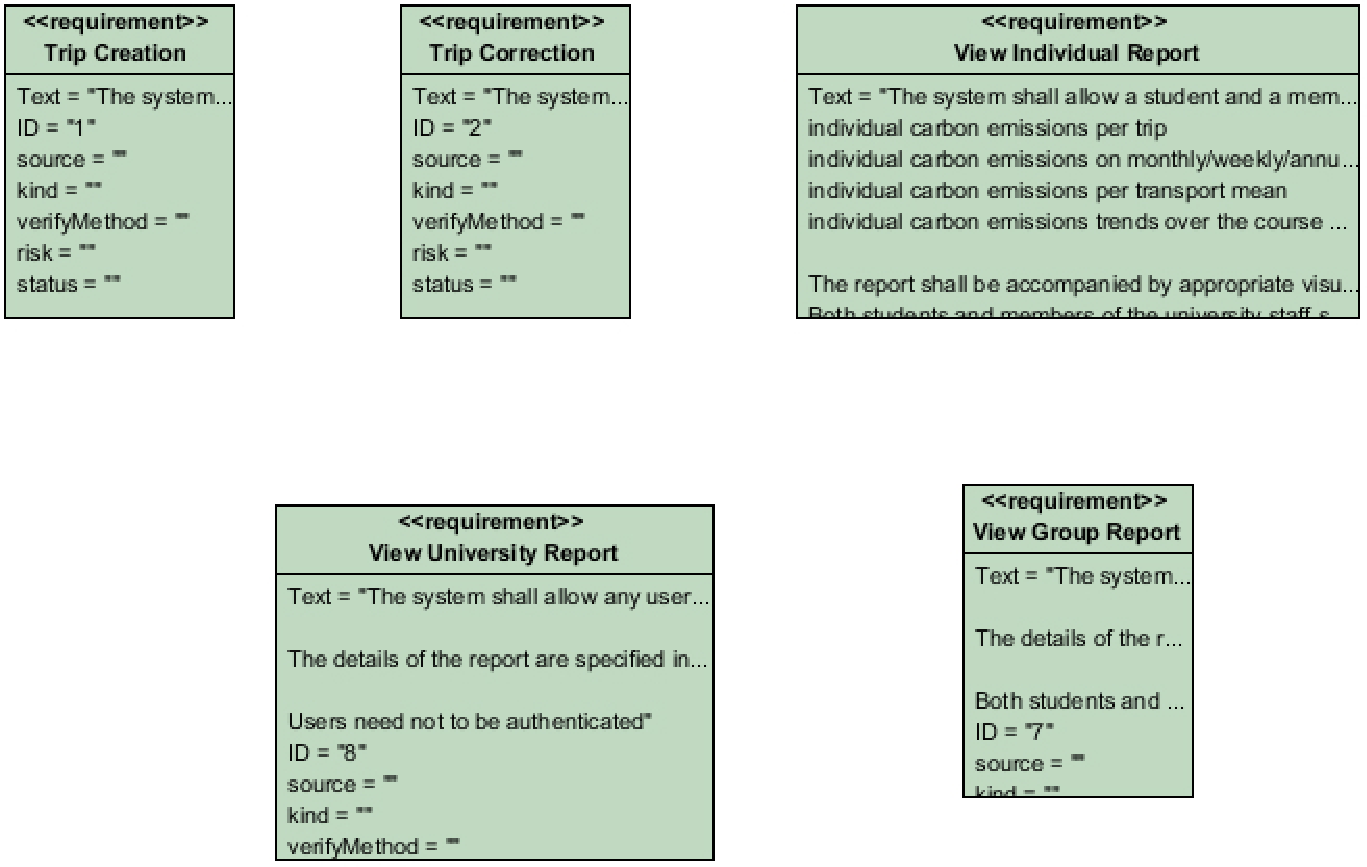
\includegraphics[scale=0.60]{./Figures/chapter4/figure1.pdf}
		\rule{35em}{0.5pt}
	\caption[System requirements diagram]{System requirements diagram}
	\label{fig:sysRequirementsDiagram}
\end{figure}

Expanding on the diagram depicted in figure \ref{fig:sysRequirementsDiagram} we can view the following requirements.

\begin{description}
  \item[Trip Creation : Requirement]
        The system shall allow a student or a member of the staff to add a new trip, by providing the appropriate information, such as, source and destination of the trip, as well as, the transport mean that was used. A user must be authenticated before adding a new trip.
  \item[Trip Correction : Requirement]
        The system shall allow a student or a member of the university staff to edit a trip that he has already created. This action demands users to be authenticated.
  \item[ View Individual Report : Requirement]
        The system shall allow a student and a member of the university staff to view his individual report presenting his carbon footprints. The report shall present:

        \begin{enumerate}
          \item individual carbon emissions per trip
          \item individual carbon emissions on monthly/weekly/annual basis
          \item individual carbon emissions per transport mean
          \item individual carbon emissions trends over the course of time
        \end{enumerate}

        The report shall be accompanied by appropriate visualization elements (e.g. charts etc.).
  \item[View Group Report : Requirement]
        The system should allow a student and a member of the university staff to view carbon emission report, concerning the groups that they are member of (e.g. research groups etc.).
        Both students and members of the university have to be authenticated.
  \item[View University Report : Requirement]
        The system shall allow any user to view a summary report about the carbon emissions of the entire university.
        Users need not to be authenticated.
\end{description}


\subsection{Use Cases}

Finding the requirements was the first step. The next step is to fing use cases of the application. Figure \ref{fig:useCasesDiagram} illustrates a diagram with the system's use cases. A description of each use case is summarized in table \ref{useCases} further below along with the corresponding flow of events.

\begin{figure}[htbp]
	\centering
		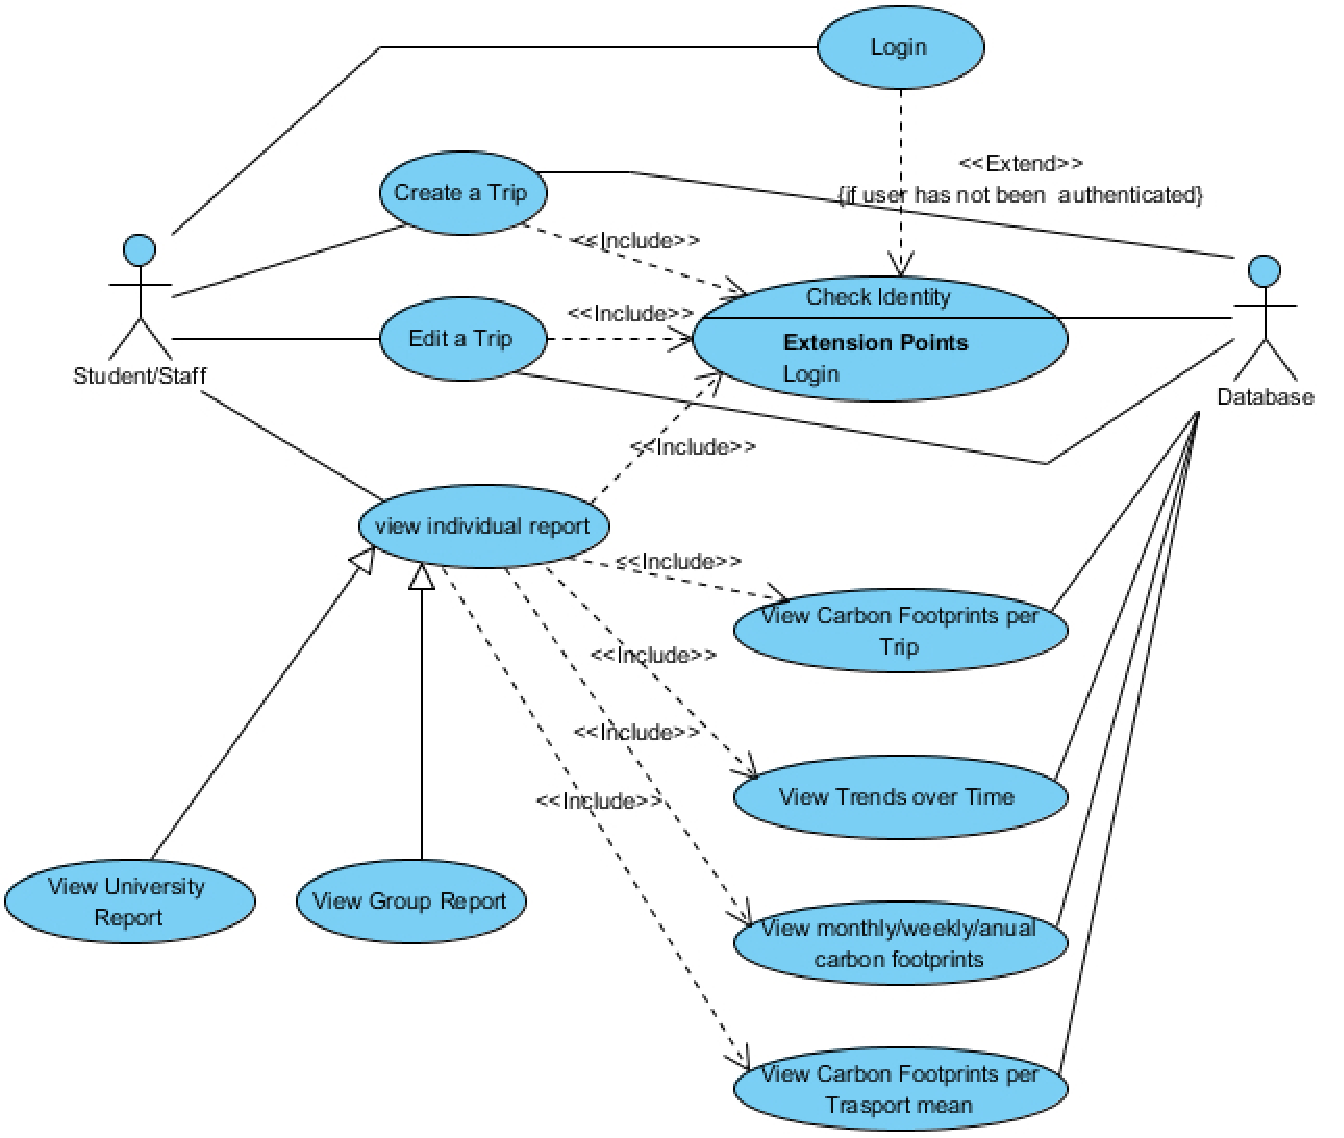
\includegraphics[scale=0.60]{./Figures/chapter4/figure2.pdf}
		\rule{35em}{0.5pt}
	\caption[Use cases diagram]{Use cases diagram}
	\label{fig:useCasesDiagram}
\end{figure}

\begin{description}
  \item[Student/Staff : Actor]
        Students or members of university staff.
  \item[Database : Actor]
        The persistent storage where all the data are stored.
  \item[Create a Trip : Use Case]
        A use case where authenticated users can add trips they made, by providing the appropriate details.
  \item[Check Identity : Use Case]
        A process that assures that specific operations can only be executed by authenticated users.
  \item[Edit a Trip : Use Case]
        A use case indicating that an authenticated user (i.e. a student or a member of the staff) can modify the details of a trip that she has added to the system.
  \item[Login : Use Case]
        A use case where users provide their credentials in order to enter the system and are able to execute operations that require them to be authenticated (e.g. trip creation).
  \item[view individual report : Use Case]
        A use case where authenticated users (i.e. students or members of the university staff) can view their individual carbon emissions report trough a rich web UI.
  \item[View Carbon Footprints per Trip : Use Case]
        A use case where authenticated users (e.g. students and members of university staff) can view the carbon emitted by each of the trips they have made.
  \item[View monthly/weekly/anual carbon footprints : Use Case]
        A use case where authenticated users (e.g. students and members of university staff) can view the carbon emissions caused by their travel activities, on weekly, daily or annual basis.
  \item[View Trends over Time : Use Case]
        A use case where authenticated users (e.g. students and members of university staff) can view their carbon emissions over the course of time, through appropriate web UI widgets (e.g charts).
  \item[View Carbon Footprints per Trasport mean : Use Case]
        A use case where authenticated users (e.g. students and members of university staff) can view the carbon emissions categorized by the transport means that were used.
  \item[View Group Report : Use Case]
        A use case where authenticated users can view the carbon emissions report for the groups that they are members of.
  \item[View University Report : Use Case]
    	A use case where any user can view carbon emissions report about a university.
\end{description}



\subsubsection{Flow of Events}

Each use case comprise a number of actions that needs to be executed. We therefore, strived to locate those steps way before the implementation part was started. We provide the flow of events for our use cases, in the following lines.

\paragraph{Create a Trip : Use Case}
\mbox{}\\
\newline
\textcolor[rgb]{0.00,0.00,1.00}{\textbf{Steps}}

\begin{verbatim}
1.  The user asks the system to create a new trip
2.  Check Identity
3.  The system asks the user to add the source and destination of the trip,
    as well as, the transport mean that was used. For each of those fields,
    the system might let the user to choose from some pre-defined values
    (e.g. common addresses and transport means) that had been configured
    by the user.
4. The user provides all the required information and submits the form.
    4.1. The user adds the source and destination address of the trip
        4.1.1. if The address exist in the system
            4.1.1.1. if the user wants to select a private address
                    (i.e. addresses had bee added by the user in the past)
                4.1.1.1.1. The user selects an address from the list of private
                           addresses
                4.1.1.1.2. The system shows the address on a map
                4.1.1.1.3. The user confirms the address or picks a different
            4.1.1.2. else
                4.1.1.2.1. The user selects an address from the list of public
                           addresses
                4.1.1.2.2. The system shows the address on a map
                4.1.1.2.3. The user confirms the address or picks a different
                     end if
        4.1.2. else
            4.1.2.1. The users chooses to add a new address
            4.1.2.2. The system shows the address creation form
            4.1.2.3. The user enters the address
            4.1.2.4. The user specifies the visibility of the address
                    (i.e. private or public)
            4.1.2.5. The user click the add address button
            4.1.2.6. The system stores the address into the persistent storage
               end if
    4.2. The user adds the transport mean
        4.2.1. The user selects the type of the transport mean
              (e.g. car, bus, taxi etc.)
        4.2.2. if the user selected the car option
            4.2.2.1. if the user wants to select one of the cars he stored into
                     the system
                4.2.2.1.1. the system show all the cars that the user stored in
                     the system
                4.2.2.1.2. the user selects a car
            4.2.2.2. else
                4.2.2.2.1. The system show a car creation form
                4.2.2.2.2. The user adds some the information about the car
                           (e.g. engine capacity,name etc. )
                4.2.2.2.3. The system add the car to the list of cars that have
                           been used by the user
                     end if
        4.2.3. else
            4.2.3.1. The user selects the specific type of transport mean
               end if
5. The user add the date and time of the trip
6. A new trip is created and inserted into the persistent storage.
\end{verbatim}


\paragraph{Edit a Trip : Use Case}

\mbox{}\\
\newline
\textcolor[rgb]{0.00,0.00,1.00}{\textbf{Steps}}

\begin{verbatim}
1. The user asks the system to edit a trip
2. Check Identity
3. The system retrieves from the persistent storage, the the trips that
   has been added by the user. Trips should be easily searchable, so that
   users can easily locate the one they want to alter.
4. The user selects the trip she wants to modify
5. The system presents a form populated with the details about the
   selected trip.
6. The user modifies the trip details and submits the form
7. The modified trip record is stored back to the persistent storage
\end{verbatim}

\paragraph{Login : Use Case}

\mbox{}\\
\newline
\textcolor[rgb]{0.00,0.00,1.00}{\textbf{Steps}}

\begin{verbatim}
1. while User is not authenticated
    1.1. The systems asks the user to provide with her credentials
    1.2. The user enters her credential
    1.3. The system checks if the given data exist in the database
    1.4. The system authenticates the user
   end while
\end{verbatim}

\textcolor[rgb]{0.00,0.00,1.00}{\textbf{Extension}}
\begin{verbatim}
1.3.a. Authentication Failure
    1. The system cannot find user's credential in the database
    2. An error message is displayed
    3. jump to 1.1. The systems asks the user to provide with her credentials
\end{verbatim}

\paragraph{Check Identity : Use Case}

\mbox{}\\
\newline
\textcolor[rgb]{0.00,0.00,1.00}{\textbf{Steps}}

\begin{verbatim}
1. The system checks if the given user has already been authenticated
2. The system allow the user to execute the operations that need
   authentication
\end{verbatim}

\textcolor[rgb]{0.00,0.00,1.00}{\textbf{Extension}}
\begin{verbatim}
1.a. Login
\end{verbatim}


\paragraph{View individual report : Use Case}

\mbox{}\\
\newline
\textcolor[rgb]{0.00,0.00,1.00}{\textbf{Steps}}

\begin{verbatim}
1. The user asks the system to view her individual carbon emissions report
2. Check Identity
3. The system presents the individual report for the user
    3.1. View Carbon Footprints per Trip View monthly/weekly/anual carbon
    footprints View Trends over Time View Carbon Footprints per Trasport mean
\end{verbatim}


\subsubsection{Activity Diagrams}

The flow of events for each use case that we oulined earlier, can be better illustrated with the aid of UML Activity Diagrams that follows.

\begin{figure}[htbp]
	\centering
		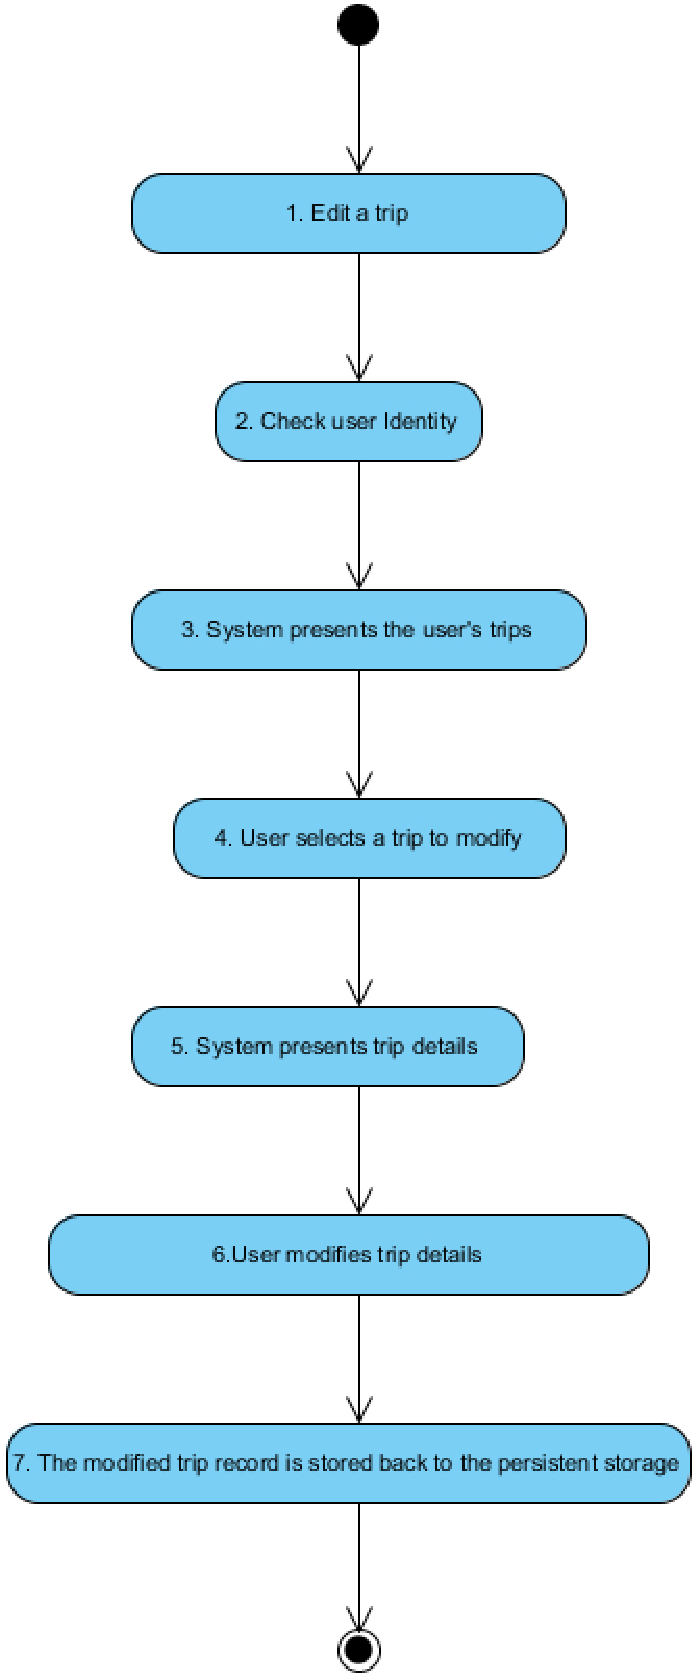
\includegraphics[scale=0.80]{./Figures/chapter4/figure3.pdf}
		\rule{35em}{0.5pt}
	\caption[Edit trip activity diagram]{Edit trip activity diagram}
	\label{fig:activityDiagramEditTrip}
\end{figure}


\begin{figure}[htbp]
	\centering
		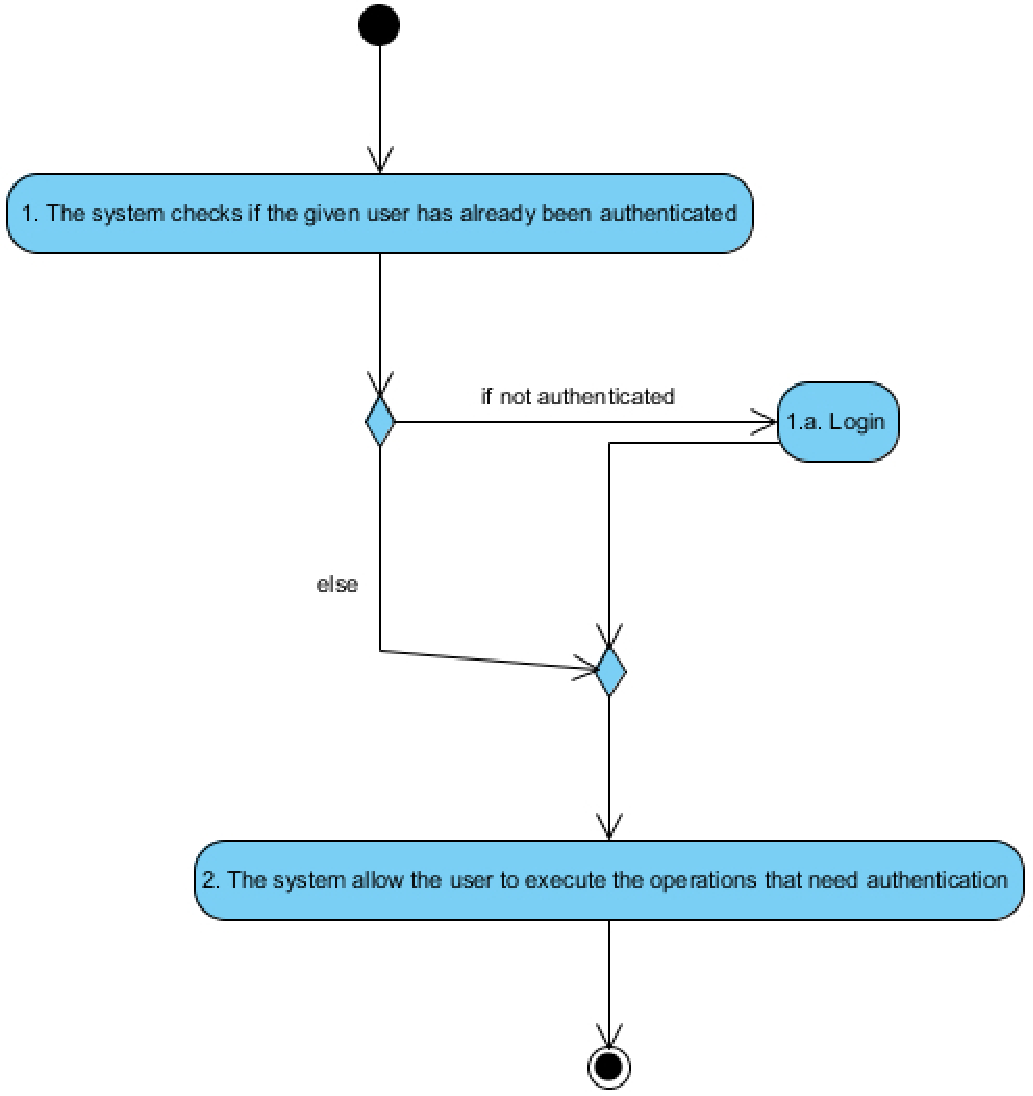
\includegraphics[scale=0.80]{./Figures/chapter4/figure4.pdf}
		\rule{35em}{0.5pt}
	\caption[Check identity activity diagram]{Check identity activity diagram}
	\label{fig:activityDiagramCheckIdentity}
\end{figure}

\begin{figure}[htbp]
	\centering
		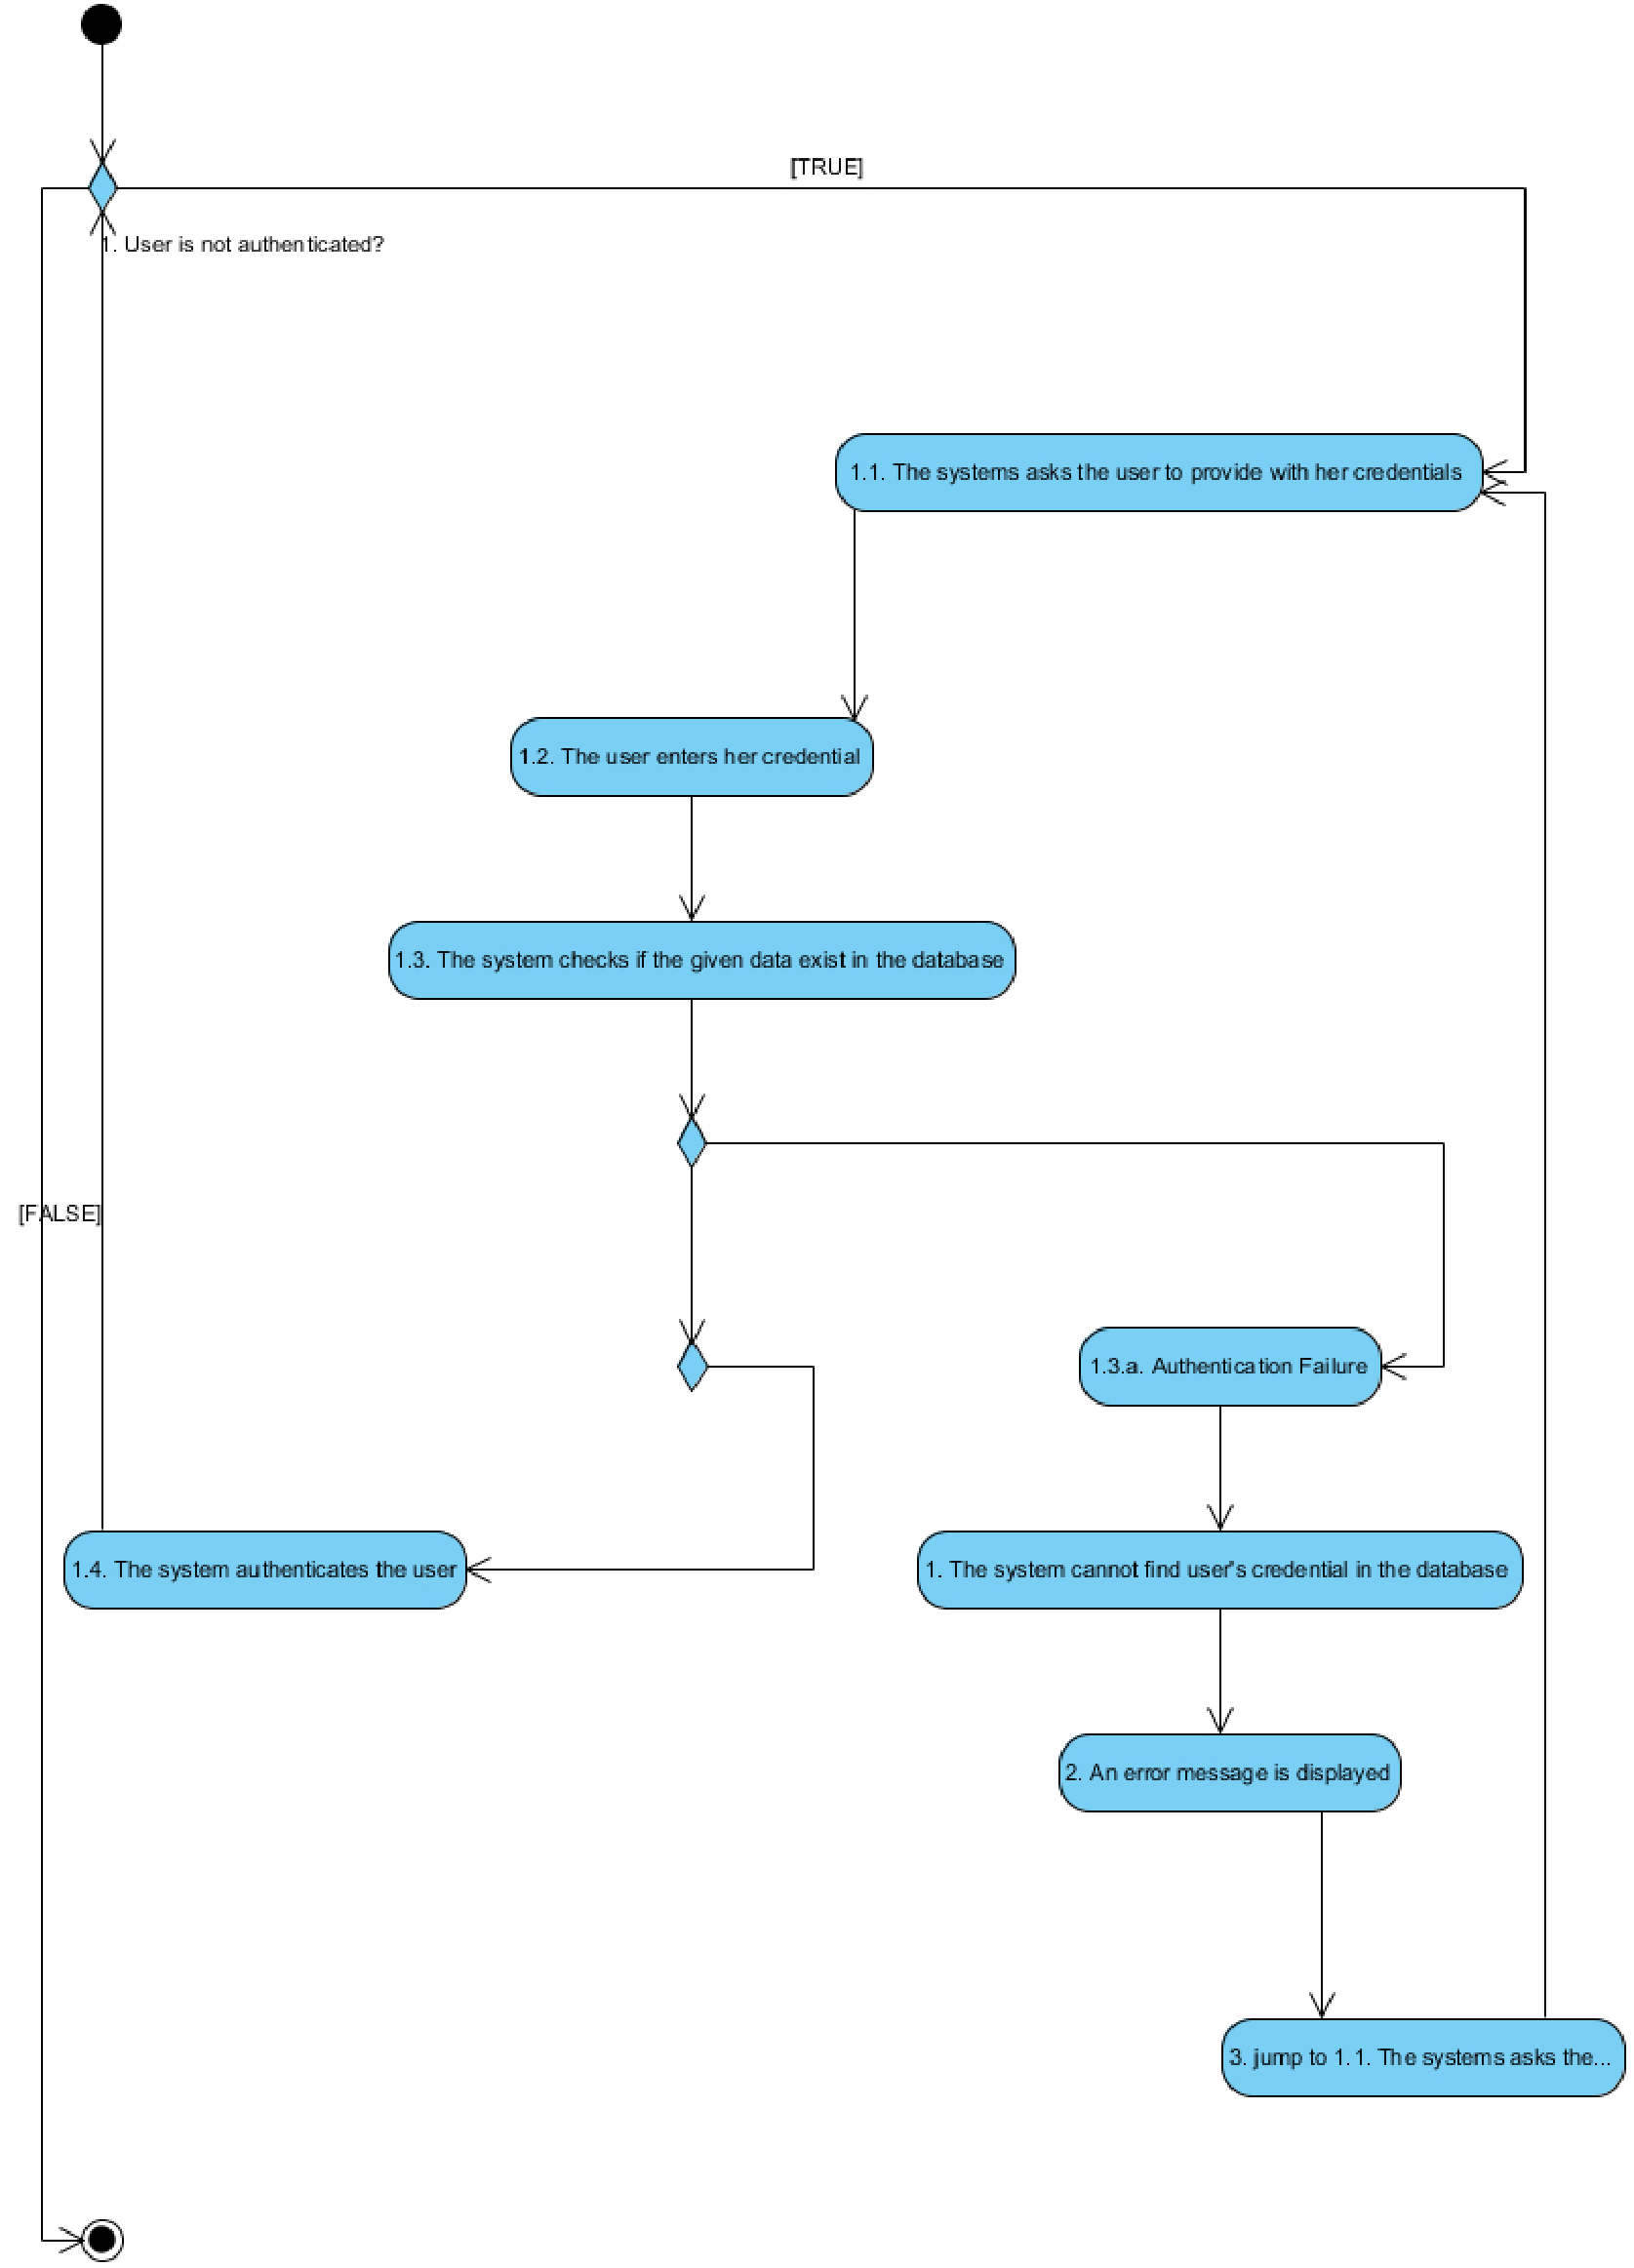
\includegraphics[scale=0.50]{./Figures/chapter4/figure5.pdf}
		\rule{35em}{0.5pt}
	\caption[Login activity diagram]{Login activity diagram}
	\label{fig:activityDiagramLogin}
\end{figure}


\subsection{Class Diagrams}

The code of the application both on back-end and front-end was written in object oriented languages (though javascript is not pure object oriented language); therefore, what follows are class diagrams for the back and front-end.

\subsubsection{Back End}

Figure \ref{fig:backEndClassDiagram} shows the back end class diagram and table \ref{backEndClasses} summarizes brief descriptions for each class.

\begin{figure}[htbp]
	\centering
		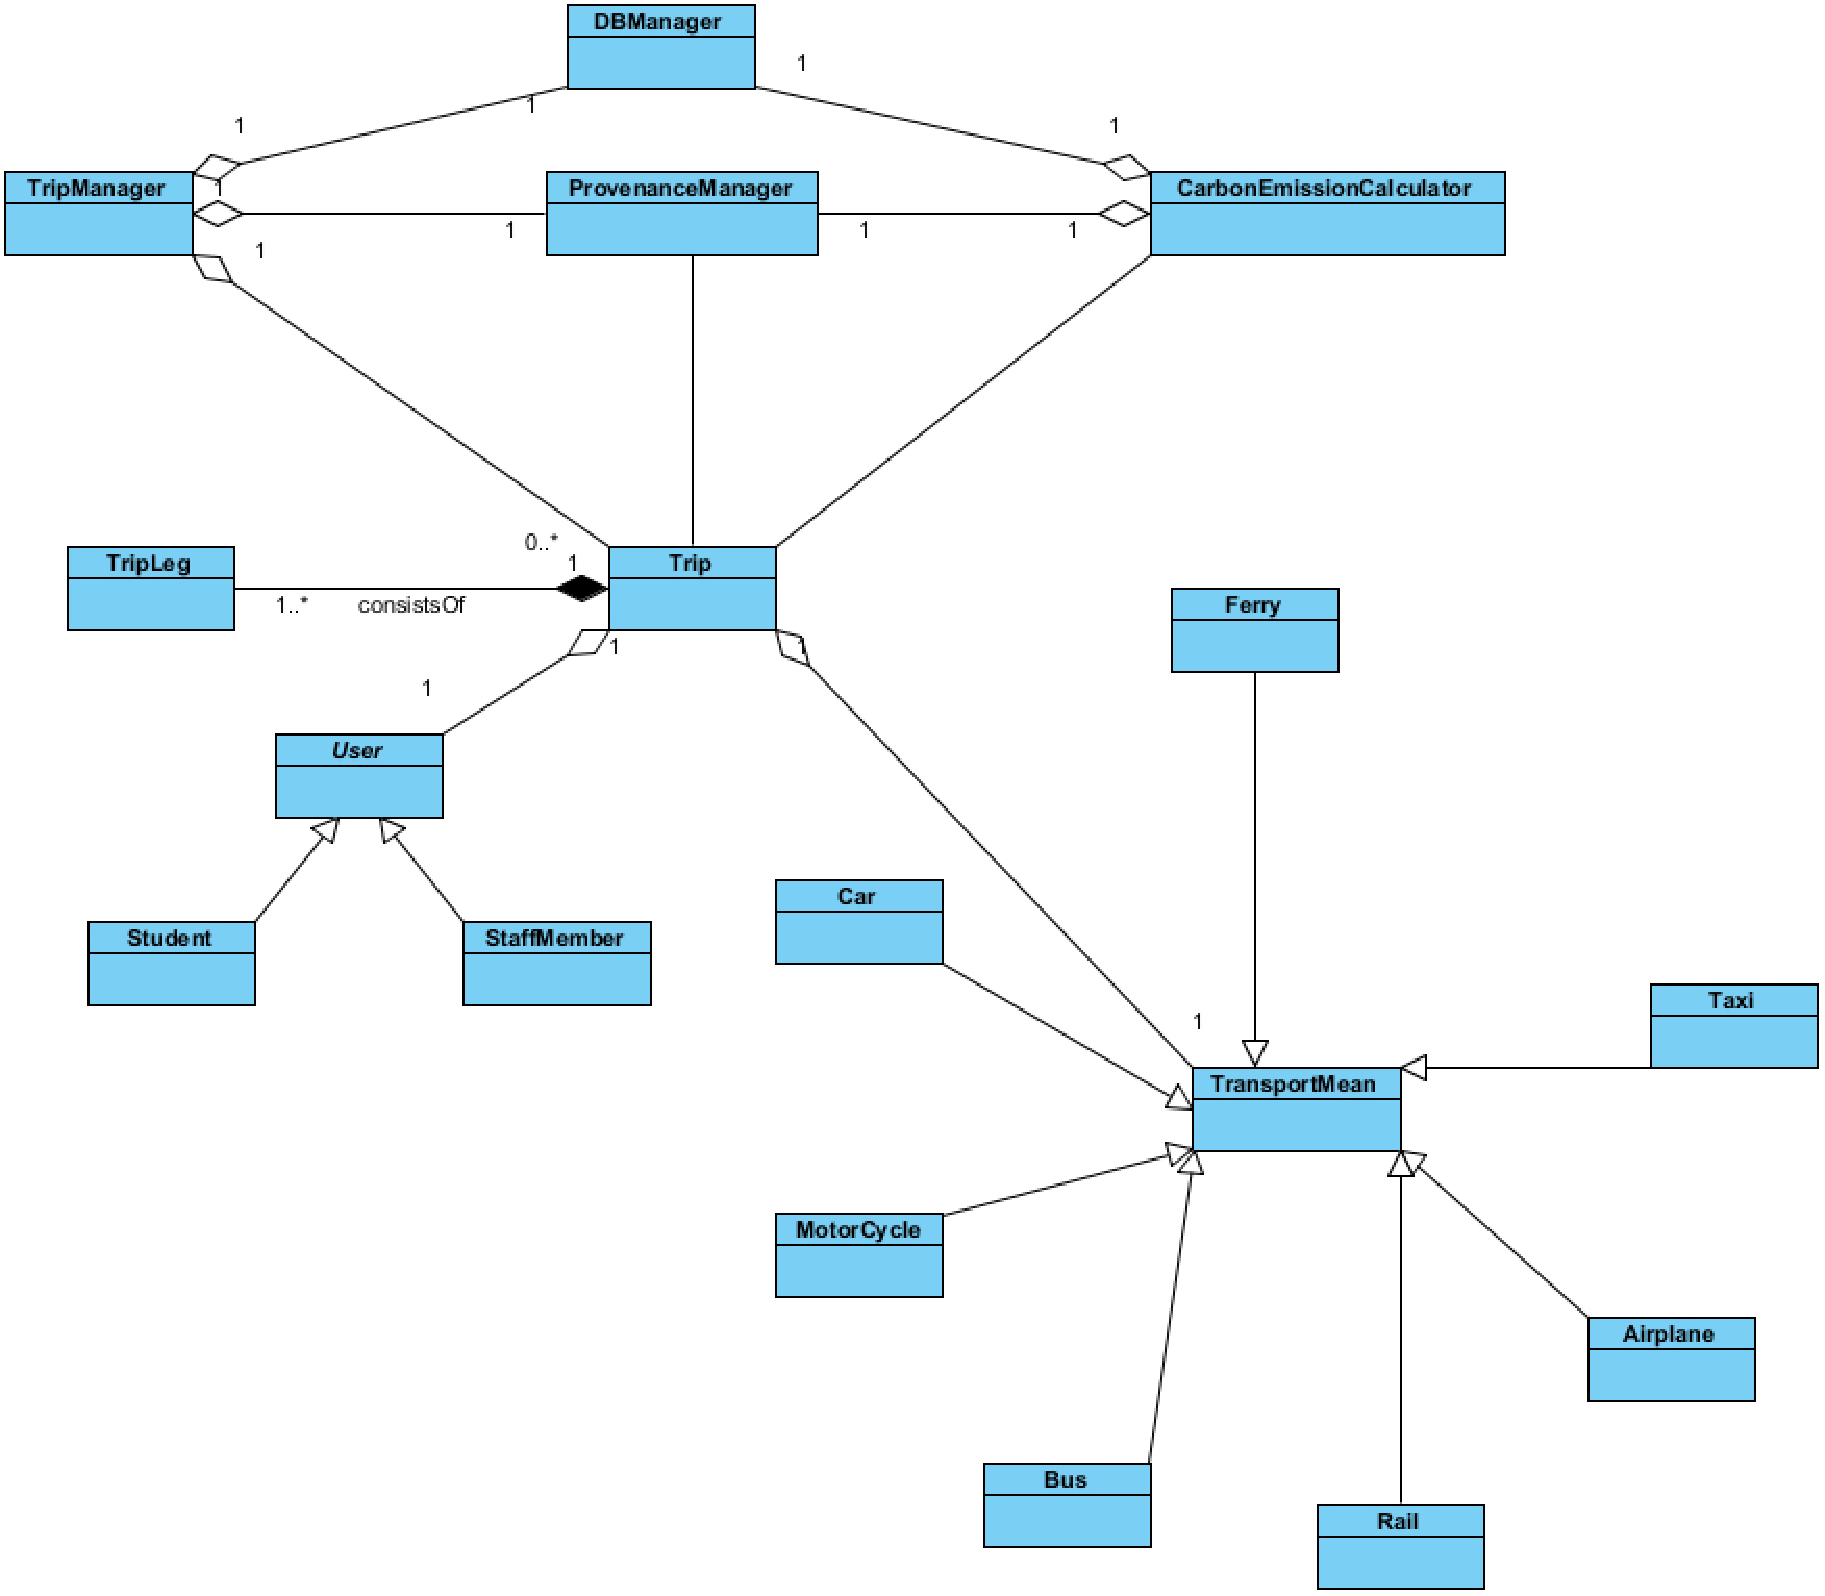
\includegraphics[scale=0.50]{./Figures/chapter4/figure6.pdf}
		\rule{35em}{0.5pt}
	\caption[Back-end class diagram]{Back-end class diagram}
	\label{fig:backEndClassDiagram}
\end{figure}

\begin{table}
  \centering
  \begin{tabular}{|p{150px}|p{250px}|}
    \hline
    Class  & Description\\
    \hline
    Trip & The main enity of the application. It represents the trip that users make. \\
    TripLeg & Each trip can have several intermediary step. Trip legs represents those steps \\
    TransportMean & The class represents transport means that are used during user's trips. It is an abstract class which has concrete subclasses (i.e Car, Motorcycle etc.) \\
    User & instances of this class refer to the user of our application. \\
    TripManager & A class responsible for all the tasks concerning user trips management, such as trip addition, trip modification etc. \\
    ProvenanceManager & A class responsible for provenance-related tasks, such as creation, storing etc. of provenance graphs. \\
    CarbonEmissionCalculator & A class responsible for calculating the carbon emissions of trips, trip legs etc. \\
    DBManager & A class responsible for database-related tasks. To be accurate, this is an ORM tool provided by the Django framework for supporting object relation mapping. \\
    \hline
  \end{tabular}
  \caption{Back-end classes}\label{backEndClasses}
\end{table}

\subsubsection{Front-End}

Our application has several tasks that are executed on client side. More specifically, the application employs the MVC using the Ember.js framework. Thus, the client-side code consists of the core constituents of the MVC pattern that is, models, views and controllers. Views are the classes which users interact with via the corresponding html template, whereas models are the actual data that the application holds. Finally, controllers are the connections between views and models.

We will separate the front-end class diagram into three figures. The first diagram (figure \ref{fig:frontEndClassDiagramTripManagement}) presents the classes that participate in trip management tasks, such as trip creation. The second diagram (figure \ref{fig:frontEndClassDiagramVisualizationTasks}) comprises classes that participate in data visualization-related tasks, such as chart and graph presentation. Finally, the third diagram (figure \ref{fig:frontEndClassDiagramUserTripPresentationTask}) illustrates the classes that take part in the user trip presentation task.


\begin{figure}[htbp]
	\centering
		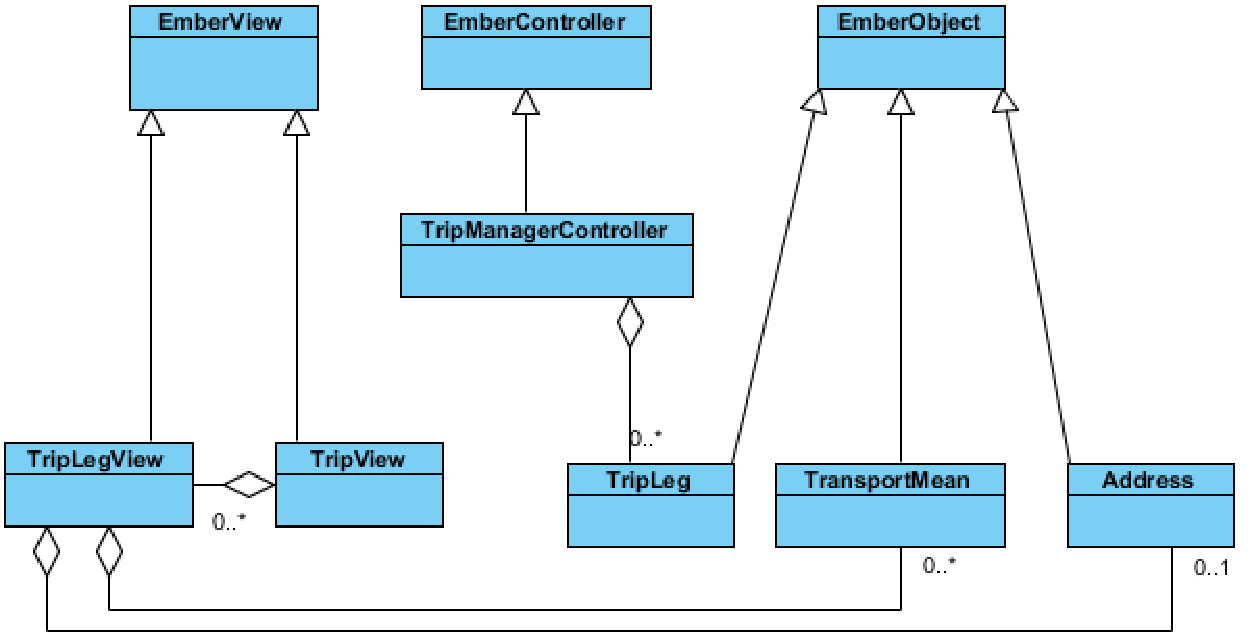
\includegraphics[scale=0.70]{./Figures/chapter4/figure7.pdf}
		\rule{35em}{0.5pt}
	\caption[Front-end class diagram comprising classes used in trip management tasks]{Front-end class diagram comprising classes used in trip management tasks}
	\label{fig:frontEndClassDiagramTripManagement}
\end{figure}

\begin{figure}[htbp]
	\centering
		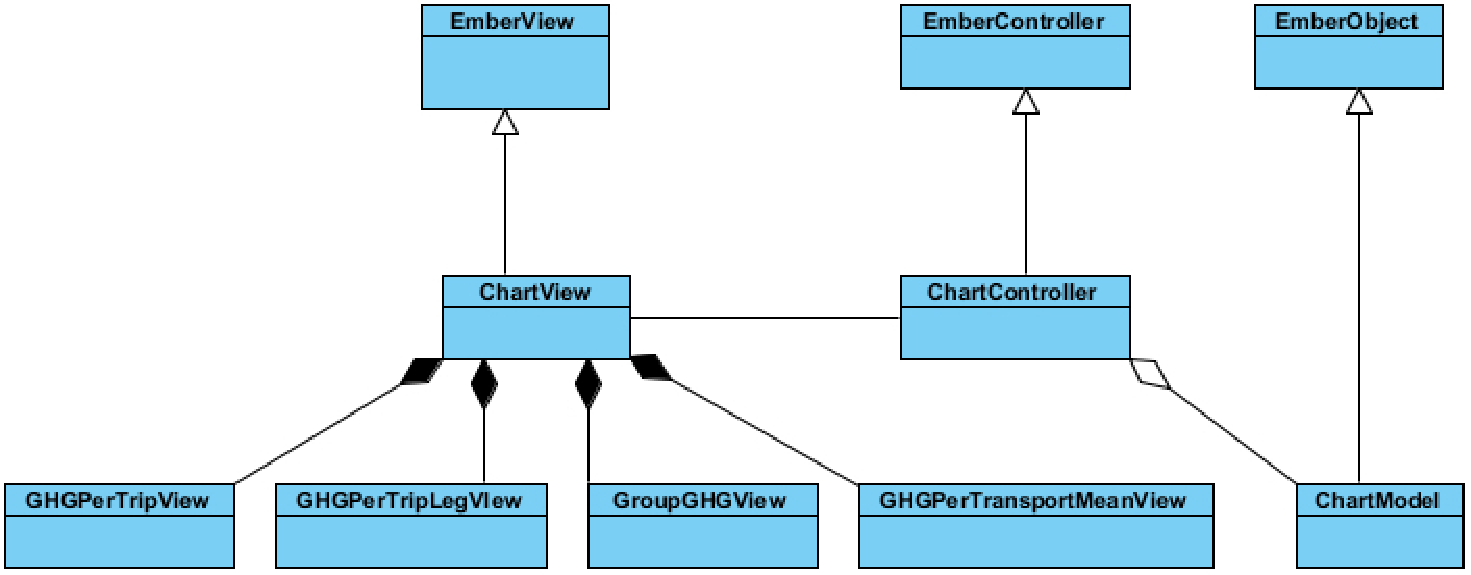
\includegraphics[scale=0.70]{./Figures/chapter4/figure8.pdf}
		\rule{35em}{0.5pt}
		\caption[Front-end class diagram comprising classes used in data visualization tasks]{Front-end class diagram comprising classes used data visualization tasks}
	\label{fig:frontEndClassDiagramVisualizationTasks}
\end{figure}

\begin{figure}[htbp]
	\centering
		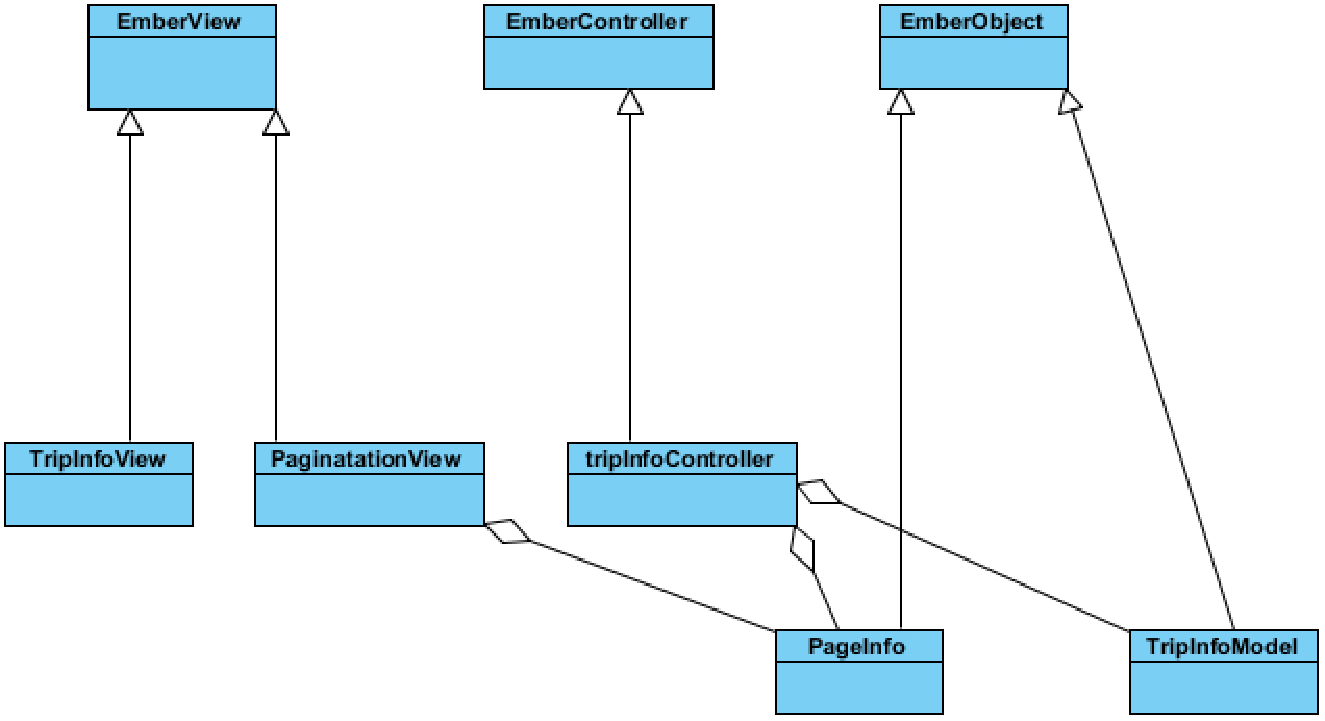
\includegraphics[scale=0.70]{./Figures/chapter4/figure11.pdf}
		\rule{35em}{0.5pt}
		\caption[Front-end class diagram comprising classes used in user trips presentation task]{Front-end class diagram comprising classes used in user trips presentation task}
	\label{fig:frontEndClassDiagramUserTripPresentationTask}
\end{figure}

\begin{table}
  \centering
  \begin{tabular}{|p{150px}|p{250px}|}
    \hline
    Class  & Description\\
    \hline
    EmberView & A class which represents views as defined by the Ember\footnote{$http://emberjs.com/$} library (Ember.View). \\
    EmberController & A class which represents controllers as defined by the Ember library (Ember.Controller). \\
    EmberObject & A class which represents models as defined by the Ember library (Ember.Object). \\
    TripManagerController & A controller responsible for gathering trip informations and sending them to the back end via AJAX Post call. \\
    TripView & A view that has an html template (i.e. html form elements) for adding information about trips. \\
    TripLegView & A view that has an html template (i.e. html form elements) for adding information about trip legs (e.g. source address, transport mena etc.). It is a sub view of the TripVew view. \\
    TripLeg & A model holding information about trip legs. \\
    TransportMean & A model that holds information about transport means. \\
    Address & A model that holds information about geographical addresse. \\
    ChartView & A view that has an html template for displaying several charts. Those charts are hosted within GHGPerTripView, GHGPerTripLegView, GroupGHGView, GHGPerTransportMeanView views. \\
    ChartModel & A model containing appropriate data that are passed as input to a JavaScript charting library. \\
    TripInfoView & A view that has an html template for displaying the trips that a used has done. \\
    PaginationView & A view containing a paginator\footnote{$http://en.wikipedia.org/wiki/Pagination$}, which helps to navigate through a list of trips. \\
    tripInfoController & A controller that fetched information about trip from the back-end via AJAX GET requests. \\
    TripInfoModel & A model containing information about trips. \\
    PageInfo & A model containing information that are required by the paginator. \\
    \hline
  \end{tabular}
  \caption{Front-end classes}\label{frontEndClasses}
\end{table}


\subsection{Database Schema}

The data model for our ampliation was probably the most important part, after capturing the requirements and forming the use cases. The application stores all data in a relational database which consists of 48 relations. More specifically, there are three sets of tables for different reasons. There is a set of tables supporting the authentication and authorization mechanism; another set used for storing provenance information; and finally a third set of tables storing the rest data produced by the application (e.g. user trips, carbon emissions, transport means etc.). Figure \ref{fig:databaseSchema} presents the database schema including tables of the third set. A brief description for each table is summarizes in table \ref{databaseTables}. Note that the database schema is missing several other tables which share similar features, such as all the other modes of transports apart from cars and their corresponding carbon emissions.

\begin{landscape}
    \begin{figure}[htbp]
	\centering
		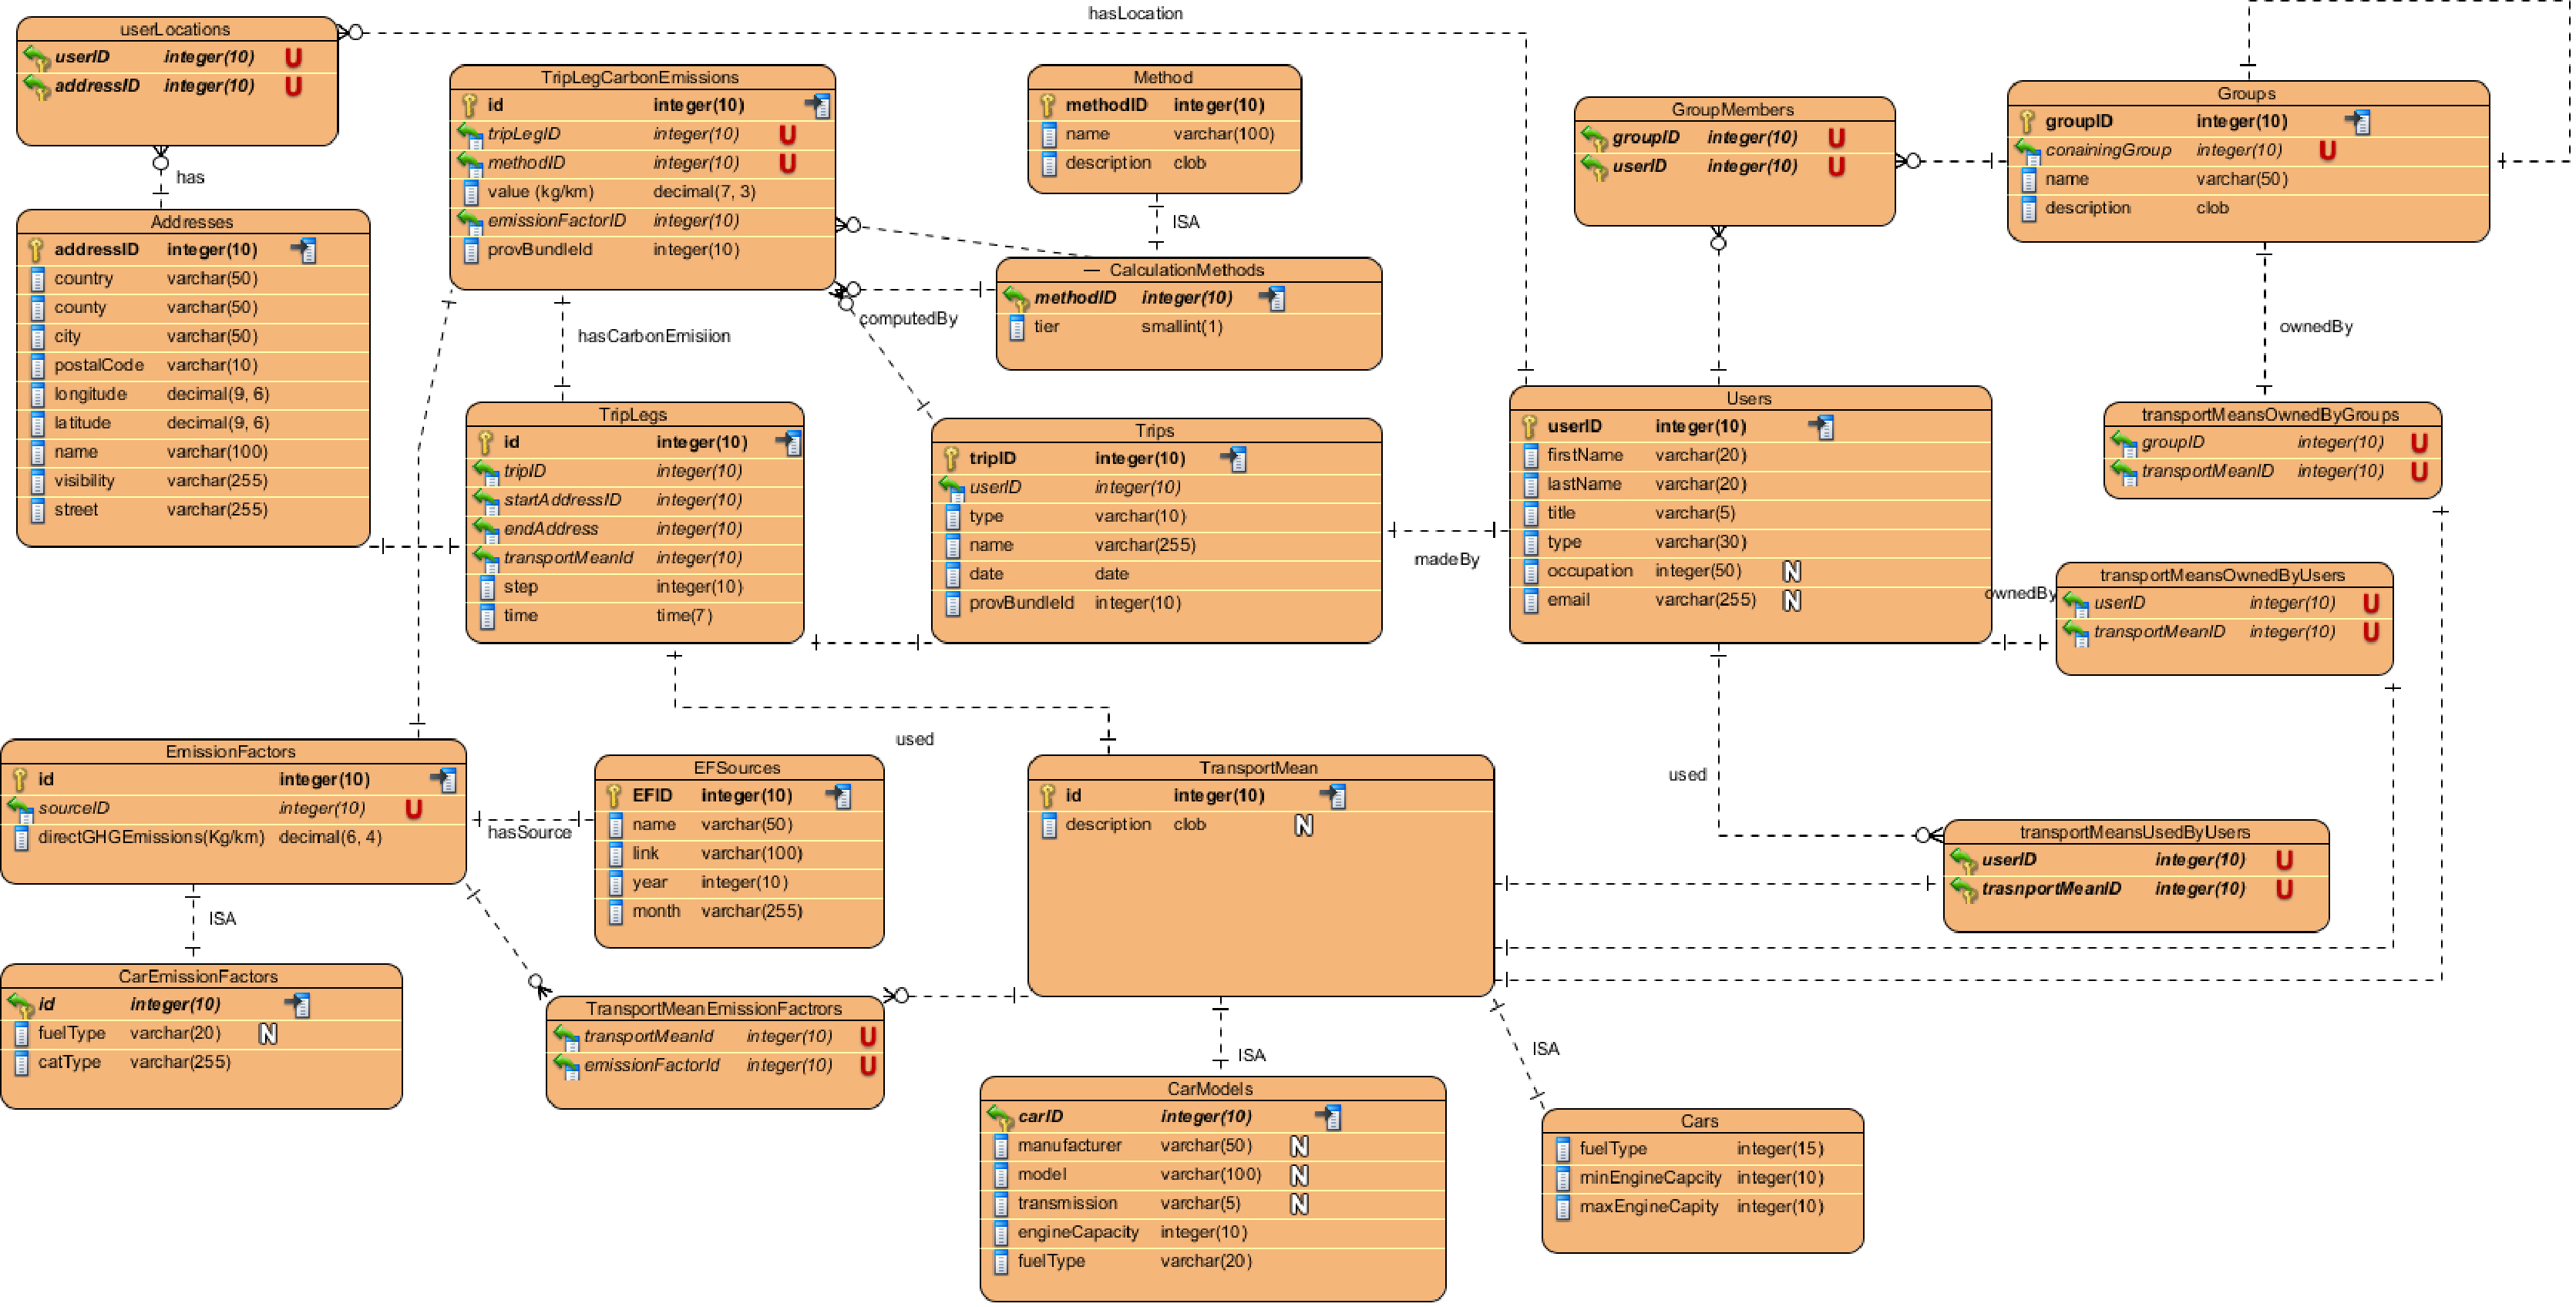
\includegraphics[scale=0.43]{./Figures/chapter4/figure9.pdf}
		\rule{35em}{0.5pt}
	\caption[Database schema]{Database schema}
	\label{fig:databaseSchema}
\end{figure}
\end{landscape}

\begin{table}
  \centering
  \begin{tabular}{|p{150px}|p{250px}|}
    \hline
    Relation  & Description\\
    \hline
    Trips & Table containing the trips made by students and the members of the university staff. \\ \hline
    TripLegs & Table storing the intermediary steps of a trip. \\ \hline
    TripLegCarbonEmissions & Table containing the calculated value of carbon emissions caused by trip legs. \\ \hline
    Method & Table containing description about different sort of methods employed by the application. For example, an extrapolation method for calculating the annual carbon emissions for an individual, based on partial set of trips that were added. \\ \hline
    CalculationMethos & Special case of the Method relation. It contains various methods for calculating carbon emissions. \\ \hline
    UserLocations & A table containing the locations that user has visited. \\ \hline
    Addresses & Table containing details about geographical addresses. \\ \hline
    TransportMean & A abstract relation that has concrete relations storing different modes of transports. CarsModels and Cars and is an example of such concrete relation. \\ \hline
    EmissionFactors &  A abstract relation that has concrete relations storing emission factors for different modes of transports. CarEmissionFactors is an example of such concrete relation \\ \hline
    TransportMeanEmissionFactors & A many-to-many relation between emission factors and transport means. Each transport mean can have different emission factors based in the source that provides them. \\ \hline
    EFSource & Table containing the sources of emission factors (e.g. IPCC etc.) \\ \hline
    Users & Table containing the users of our application. \\ \hline
    Groups & Any group that contains a number of people, such as a research group, an academic unit or the entire university. \\ \hline
    GroupMembers & Table containing the members (users) of each group. \\ \hline
    TransportMeansUsedByUsers & Table contains the transport that users have used. \\ \hline
    TransportMeansOwnedByUsers & Table contains transport means that users own. \\ \hline
    TransportMeansOwnedByGroups & Table contains transport means owned by groups. \\

    \hline

  \end{tabular}
  \caption{Database tables}\label{databaseTables}
\end{table}

\section{Summary}

In this chapter we went through the application's design phase. To make the description more obvious, various types of UML diagrams were given illustrating the path we followed towards implementing the application.

